\documentclass[12pt,utf8,notheorems,compress]{beamer}

\usepackage[ngerman]{babel}

\usepackage{amsmath,amssymb}
\usepackage{tabto}

\setlength\parskip{\medskipamount}
\setlength\parindent{0pt}

\title{Kryptographie}
\author[Matheschülerzirkel Augsburg]{Matheschülerzirkel Augsburg}
\date{15. März 2014}

%\usetheme{Warsaw}  %Warsaw, Berkeley?
\usetheme{Warsaw}
\useoutertheme{split}
\usecolortheme{seahorse}
\usefonttheme{serif}
\usepackage{palatino}
\useinnertheme{rectangles}

\setbeamertemplate{navigation symbols}{}
%\setbeamertemplate{footline}{}
%\setbeamertemplate{headline}{}

%\beamertemplateboldcenterframetitle
%\setbeamerfont{frametitle}{size={\Large}}

\newcommand*\oldmacro{}%
\let\oldmacro\insertshorttitle%
\renewcommand*\insertshorttitle{%
  \oldmacro\hfill\insertframenumber\,/\,\inserttotalframenumber\hfill}

\newcommand{\floatbox}[3]{%
  \raisebox{0pt}[0pt][0pt]{%
    \begin{picture}(0,0)(#1,#2)#3\end{picture}\leavevmode%
  }%
}

\newenvironment{changemargin}[2]{%
  \begin{list}{}{%
    \setlength{\topsep}{0pt}%
    \setlength{\leftmargin}{#1}%
    \setlength{\rightmargin}{#2}%
    \setlength{\listparindent}{\parindent}%
    \setlength{\itemindent}{\parindent}%
    \setlength{\parsep}{\parskip}%
  }%
  \item[]}{\end{list}}

\begin{document}

\frame{
  \titlepage
  \floatbox{-270}{20}{
\includegraphics[scale=0.1]{../cover}}
}

\frame[plain]{\begin{center}
  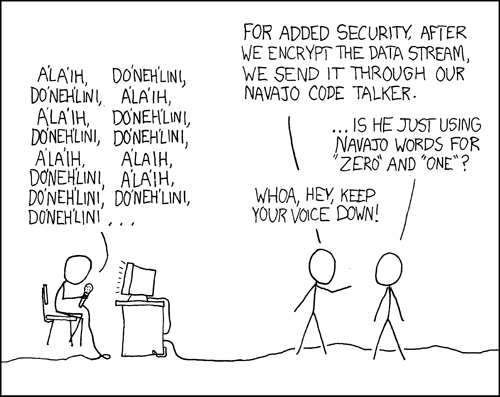
\includegraphics[scale=5]{images/code_talkers.png}

  \url{http://xkcd.com/257/}
\end{center}}

\section[Caesar]{Caesar-Verschlüsselung}
\frame[t]{\frametitle{Caesar-Verschlüsselung}
  \begin{itemize}
    \item
      Verschlüsselung durch Rotation des Alphabets
    \item
      \begin{tabbing}
        Verschlüsselung: \= \kill
        Beispielklartext: \> \texttt{Linux macht Spass!} \\
        Verschlüsselung:  \> \texttt{OlqxA pdfkw Vsdvv!}
      \end{tabbing}
  \end{itemize}
  \vfill
  \begin{center}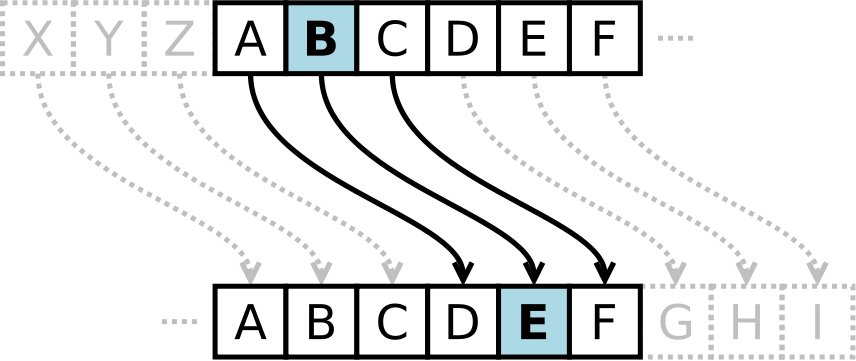
\includegraphics[scale=0.3]{images/caesar.jpeg}\end{center}
}

\section[Mono]{Monoalphabetische Substitution}
\frame[t]{\frametitle{Monoalphabetische Substitution}
  \begin{itemize}
    \item
      Verschlüsselung durch Verwendung eines Kunstalphabets
    \item
      Beispiel im Browser
  \end{itemize}
}

\section[Poly]{Polyalphabetische Substitution}
\frame[t]{\frametitle{Polyalphabetische Substitution}
  \begin{itemize}
    \item
      Verschlüsselung durch Addition, \\
      Entschlüsselung durch Subtraktion eines geheimen Schlüssels
      \floatbox{-190}{160}{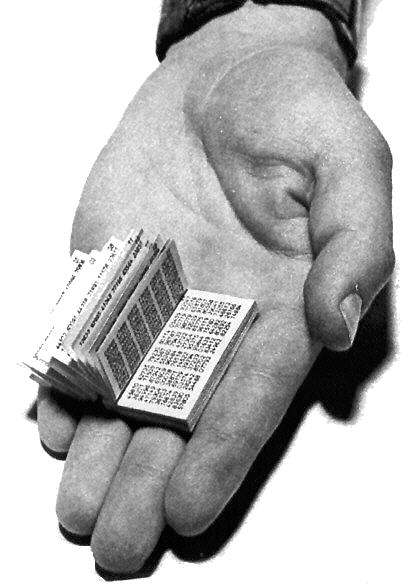
\includegraphics[scale=0.1]{images/otp.jpeg}}

    \item
      \begin{tabbing}
        Verschlüsselung: \= \kill
        Beispielklartext: \> \texttt{Linux macht Spass!} \\
        Schlüssel:        \> \texttt{GeheimerSchluessel} \\
        Verschlüsselung:  \> \texttt{RMUYf QRuJa MTSkW!}
      \end{tabbing}
  \end{itemize}
}

\section[Münzwurf]{Münzwurf über Telefon}
\frame[t]{\frametitle{Münzwurf über Telefon}
  \begin{itemize}
    \item
      Kontext: \\
      Alice und Bob telefonieren. \\
      Sie müssen entscheiden, welcher von ihnen eine unliebsame
      Aufgabe übernimmt.
      \floatbox{-70}{160}{
\includegraphics[scale=0.3]{images/coin-toss.png}}
  \end{itemize}
  \pause
  \vfill

  \begin{enumerate}
    \item Alice wählt Kopf, Bob wählt Zahl.
    \item Alice wirft eine Münze.
    \item Alice teilt Bob mit, dass die Münze Zahl anzeigt.
    \item Bob muss die Aufgabe übernehmen.
  \end{enumerate}
  \pause
  \vfill

  \begin{itemize}
    \item
      Offensichtlich: Alice kann betrügen!
  \end{itemize}
}

\section[Nullwissen]{Zero-Knowledge-Beweise}
\frame[t]{\frametitle{Zero-Knowledge-Beweise}
  \begin{itemize}
    \item
      Kontext: \\
      Alice möchte Bob davon überzeugen, dass sie ein bestimmtes Geheimnis
      kennt, ohne das Geheimnis preiszugeben.
      \floatbox{-125}{150}{%
	\only<1>{
\includegraphics[scale=0.25]{images/knowledge.jpeg}}%
	\only<2>{\hspace{1.5cm}
\includegraphics[scale=0.05]{images/schneier.jpeg}}%
      }
    \item
      Illustration: Wo ist Waldo?

    \pause
    \vfill
    \item Variante: Alice und Bob möchten \\ überprüfen, ob sie beide dasselbe \\
    Geheimnis kennen, ohne es \\ preiszugeben.
  \end{itemize}
}

\section[D--H]{Diffie--Hellman-Schlüsselaustausch}
\frame[t]{\frametitle{Diffie--Hellman}
  \begin{itemize}
    \item Kontext: \\
	  Alice und Bob wollen ohne sonstige vorherige Absprachen ein
	  gemeinsames Geheimnis ausmachen.
  \end{itemize}

  \floatbox{-190}{135}{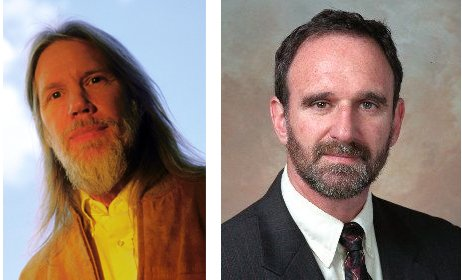
\includegraphics[scale=0.3]{images/diffie.jpeg}}
}

\appendix

\frame[t]{\frametitle{Bildquellen}
  \tiny
  \begin{itemize}
    \item \url{http://biblioragazzi.files.wordpress.com/2008/04/reference.jpg}
    \item \url{http://i34.tinypic.com/51ptu0.jpg}
    \item \url{http://imgs.xkcd.com/comics/code_talkers.png}
    \item \url{http://one-time-pad.tripod.com/otp.jpg}
    \item \url{http://upload.wikimedia.org/wikipedia/commons/2/2b/Caesar3.svg}
    \item \url{http://www.bryx.de/wp-content/uploads/2008/09/800px-zeichen_220svg.png}
    \item \url{http://www.cellphones.ca/news/upload/2008/09/knowledge1.jpg}
    \item \url{http://www.gpuri.com/images/213/21325.jpg}
    \item \url{http://www.hirt-institut.de/de/Media/Shop/CategoryTextMedia/hirt_motiv_ihre_ziele.jpg}
    \item \url{http://www.kveller.com/images/Article_images/wheres_waldo.jpg}
    \item \url{http://www.marketoracle.co.uk/images/coin-toss.jpg}
    \item \url{http://www.treachery.net/images/why_security_through_obscurity_isnt.jpg}
    \item \url{http://www.waleed-security.com/wp-content/uploads/2008/11/bruceab.jpg}
  \end{itemize}
}

\end{document}
